\documentclass[a4paper,10pt,titlepage]{scrartcl}
\usepackage[sc]{mathpazo} % Schrift - wie Funcky und in PDF zu Fonts beschrieben
\usepackage[T1]{fontenc}
\usepackage[utf8]{inputenc}
\usepackage[a-1b]{pdfx}
\usepackage[ngerman]{babel}
\usepackage[amssymb]{SIunits} 
\usepackage{graphicx} 
\usepackage{subfigure}                         
\usepackage{float}
\usepackage[iso,german]{isodate} %his package provides commands to switch between different date formats
\usepackage{hyperref}
\usepackage[left=2cm,top=1cm,right=2cm]{geometry}
\usepackage{listings}
\lstset{
    basicstyle=\tiny, %or \small
    literate=
        {Ö}{{\"O}}1
        {Ä}{{\"A}}1
        {Ü}{{\"U}}1
        {ß}{{\ss}}1
        {ü}{{\"u}}1
        {ä}{{\"a}}1
        {ö}{{\"o}}1
}

\usepackage{fancyhdr}
\renewcommand{\headrulewidth}{0.5pt}
\renewcommand{\footrulewidth}{0.5pt}
%Abstand zwischen Absätzen, Zeilenabstände
\voffset26pt 
\parskip6pt
%\parindent1cm  %Rückt erste Zeile eines neuen Absatzes ein
\usepackage{setspace}
\onehalfspacing

\begin{document}
\pagenumbering{roman}
\titlehead
{
    \small
    {
        Technische Universität Ilmenau\\
        Fakultät für Informatik und Automatisierung\\
        Institut für Biomedizinische Technik und Informatik\\

        Laborpraktikum BMT\\
        WS 2021/22}
}

\title {Versuch: Deep Learning in der Biomedizintechnik}
\subtitle{Praktikumsbetreuer: Thomas Jochmann}
\author{Teilnehmer: Robert Jeutter \& Amèle Nya}
\date{
    Datum Versuchsdurchführung: \quad 16.12.21\\
    Datum Protokollabgabe: \quad 18.12.21
}
\maketitle

%Einstellungen zur Kopf- und Fußzeile
\pagestyle{fancy}
\fancyhead[R]{Deep Learning}
\pagenumbering{arabic}
\newpage

\section{Kontrollfragen}
\begin{enumerate}
    \item Erklären Sie die Rechenschritte in einem neuronalen Netz.
          \begin{itemize}
              \item Signaleingang über Axon an Eingang des Neurons
              \item Summe aller Eingänge mti Aktivierungsfunktion (Soma) verrechnen
              \item Ausgabe der Aktivierungsfunktion mit Ausgabefunktion (Axonhügel) berechnen
              \item Ergebnis der Ausgabefunktion auf Ausgang legen
          \end{itemize}
    \item Nennen Sie drei Aktivierungsfunktionen von neuronalen Netzen.
          \begin{itemize}
              \item Skalarprodukt $\sum_{j=1}^n w_{ij} * x_J$
              \item Sigma-Pi $\sum_{j=1}^n (w_{ij} * \prod_{w=1}^p x_{jw})$
              \item Manhatten $\sum_{j=1}^n |x_j-w_{ji}|$
              \item Euklidische Distanz $\sqrt{\sum_{j=1}^n (x_j-w_{ji})^2}$
              \item Mahalanobis $\sqrt{(x-w_i)^T *C_i^{-1} * (x-w_i)}$ mit $C_i=\frac{1}{n} \sum_{p=1}^N (x^p-w_i)*(x^p-w_i)^T$
              \item Maximum-Distanz: $max_{1\leq j\leq n} |x_j-w_{ij}|$
              \item Minimum-Distanz: $min_{1\leq j\leq n} |x_j-w_{ij}|$
          \end{itemize}
    \item Nennen Sie verschiedene Arten von Layern in neuronalen Netzen.
          \begin{itemize}
              \item Input-Layer: Neuronen, die von der Aussenwelt Signale empfangen
              \item Hidden-Layer: Neuronen, die sich im inneren des neuronalen Netzes befinden und eine interne Repräsentation der Aussenwelt enthalten
              \item Output-Layer: Neuronen, die Signale an die Aussenwelt abgeben
          \end{itemize}
    \item Warum ist es nicht sinnvoll eine lineare Funktion $(y=\alpha x+b)$ als Aktivierungsfunktion in den verdeckten Schichten eines neuronalen Netzes zu verwenden?
    \item Was verstehen Sie unter Backpropagation?
          \begin{itemize}
              \item Im Wesentlichen ist Backpropagation ein Algorithmus, der zur schnellen Berechnung von Ableitungen verwendet wird
              \item auch Fehlerrückführung oder Rückwärtspropagierung
              \item um einen Gradientenabstieg in Bezug auf Gewichtungen zu berechnen
              \item gewünschte Ausgaben werden mit erreichten Systemausgaben verglichen, und dann werden die Systeme durch Anpassung der Verbindungsgewichte so eingestellt, dass der Unterschied zwischen den beiden so gering wie möglich ist
              \item der Algorithmus hat seinen Namen daher, dass die Gewichtungen rückwärts aktualisiert werden, von der Ausgabe zur Eingabe
          \end{itemize}
    \item Warum ist eine Stufenfunktion (Rosenblatt-Perceptron) ungünstig für den Backpropagation-Algorithmus?
          \begin{itemize}
              \item Anpassung schlecht möglich
          \end{itemize}
    \item Was ist die Learning Rate? Was passiert, wenn sie zu hoch oder niedrig gewählt wird?
          \begin{itemize}
              \item Sein Wert bestimmt, wie schnell das Neuronale Netz zu Minima konvergieren würde
              \item wenn er zu niedrig ist, ist der Konvergenzprozess sehr langsam
              \item wenn er zu hoch ist, ist die Konvergenz schnell, aber es besteht die Möglichkeit, dass der Verlust überschreitet
          \end{itemize}
    \item Was verstehen Sie unter Augmentation? Nennen Sie Beispiele für Augmentation.
          \begin{itemize}
              \item mit Hilfe von verschiedenen Prozessen die Originalbilddaten verändern
              \item Beispielsweise kann ein Bild gedreht werden oder es ist möglich einen Filter über das Bild zu legen
          \end{itemize}
    \item Warum ist es bei neuronalen Netzen besonders wichtig, die Testdaten beim Training außen vor zu lassen?
          \begin{itemize}
              \item Um einen korrekten Vergleich mit anderen Netzen und unabhängigkeit vom Training nachzuweisen
          \end{itemize}
    \item Wie können Sie die Güte eines neuronalen Netzes bewerten?
          \begin{itemize}
              \item Durch Vergleich der Ausgabe der verifizierten Testdaten mit realen Ergebnissen um den Unterschied zwischen Richtigen, Falsch-Richtigen, Falschen und Falsch-Richtigen Ergebnissen zu einem Wert, der Güte, zusammenzufassen
          \end{itemize}
    \item Warum ist es potentiell kritisch, wenn mit einem neuronalen Netz ein unscharfes Bild scharf und hochaufgelöst gemacht wird?
          \begin{itemize}
              \item kleine fehlerhafte oder ungenaue Bild-Sektionen können zu größeren Fehlern und Abweichungen von dem Original führen die durch die Hochauflösung überdeckt oder verschoben werden
          \end{itemize}
\end{enumerate}
\newpage

\section{Versuchsdurchführung}
\subsection{Notebook 1: Grundkenntnisse zur Anwendung von Deep Learning}
\subsubsection{Aufgabe 1a) Erstellen eines einfachen neuronalen Netzes}
Gegeben ist ein neuronales Netz (NN). Berechne von Hand mit den gegebenen Gewichten den Output des Netzes für die Inputs $x = -1, 1$ und $2$. Die Aktivierungsfunktion aller Neuronen sei 'ReLu'.

\begin{itemize}
    \item Skalarproduktaktivierung: $z_i(x_i, w_i, b)=w_i *x_i+b$
    \item ReLU: $y_i (z_i)=max(0,z_i)$
    \item Neuron $y(x,w,b)=max(0,\sum w_i*x_i+b)$
    \item $x=[-1,1,2]$
    \item $w=[3,2,1,1,-5]$
    \item $b=[0,0,-5,0]$
    \item $y_0=max(0, w_0*x_0+b_0 + w_1*x_1+b_0 + w_2*x_2+b_0) = max(0, 3*(-1)+0 +3*1+0 + 3*2+0) = max(0,-3+3+6)=6$
    \item $y_1=max(0, 2*6+0)=12$
    \item $y_2=max(0, 1*6-5)=1$
    \item $y_3=max(0, 1*12 + (-5)*1)=max(0, 12-5)=7$
\end{itemize}

Im Folgenden soll die eben gelöste Aufgabe erneut mit der Bibliothek ,,keras'' gelöst werden. Erzeuge mit Hilfe der Befehle aus der Vorbereitung das NN. Dazu werden zunächst die benötigten Bibliotheken geladen. Neue Schichten können mit dem Befehl `model.add()` hinzugefügt werden.

\begin{lstlisting}[language=python]
# Import der benötigten Bibliotheken 
exec(open(r"../data/notebook1_code.py").read())
%matplotlib inline

# Laden eines Modelltyps für das neuronale Netz
model=tf.keras.models.Sequential()

# TODO: Füge die drei benötigten Schichten zum Netz hinzu
# Hinweis: Vergessen Sie nicht im ersten Layer die Inputdimension anzugeben
model.add(tf.keras.layers.Dense(1, input_shape=(1,), activation='relu'))
model.add(tf.keras.layers.Dense(2, input_shape=(2,), activation='relu'))
model.add(tf.keras.layers.Dense(1, input_shape=(2,), activation='relu'))

# Erzeugen des NN nach der oben festgelegten Struktur
model.compile(optimizer="adam",
              loss="mean_squared_error",
              metrics=["accuracy"])
\end{lstlisting}

Das Netz enthält in dieser Form zufällig initialisierte Gewichte. Setze die Gewichte und Bias.

\begin{lstlisting}[language=python]
# TODO: Wähle die Werte der Gewichte und des Bias
w01 = 3
w11 = 2
w21 = 1
w12 = 1
w22 = -5

b1 = 0
b2 = 0
b3 = -5
b4 = 0

# Gewichte werden in das von keras geforderte Datenformat gebracht und in weight_list gespeichert
weight_list = [np.array([[w01]]),np.array([b1]),np.array([[w11, w21]]),np.array([b2, b3]),np.array([[w12], [w22]]),
               np.array([b4])]

# TODO: Übergebe die Gewichtsmatrizen (weight_list)
model.set_weights(weight_list)

\end{lstlisting}

Nutze nun die predict-Funktion, um die handschriftlichen Rechnungen zu überprüfen.

\begin{lstlisting}[language=python]
# TODO: Führe eine Prediction für drei Werte [-1, 1, 2] durch.
model.predict([-1, 1, 2])
\end{lstlisting}

Ausgabe:
\begin{lstlisting}[language=python]
array([[0.], [6.], [7.]], dtype=float32)
\end{lstlisting}

\textbf{Antwort:} Der Rechenweg und das Neuronale Netzwerk liefern dasselbe Ergebnis.

\subsubsection{Aufgabe 1b) Neuronales Netz zur Funktionsapproximation}
Statt nur einzelne Punkte zu predicten können auch größere Bereiche auf dem Zahlenstrahl abgetastet werden. Gebe dazu 50 Werte von -5 bis 5 in die predict-Funktion.

\begin{lstlisting}[language=python]
# Importieren der Bibliothek für die Darstellung der Kurve
from matplotlib import pyplot as plt

# TODO: Gebe die Werte -5 bis 5 in 50 Schritten auf die predict-Funktion und speicher die Ausgabe in der Variable result
result = model.predict(np.linspace(-5, 5, 50))

# Ausgabe der approximierten Funktion
plt.plot(np.linspace(-5,5),result)
\end{lstlisting}

Gebe das Diagramm im Protokoll an:
\begin{center}
    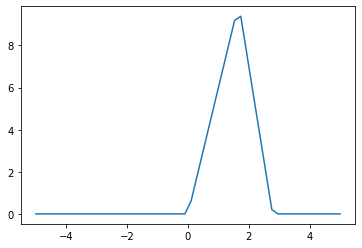
\includegraphics[width=.5\linewidth]{Assets/prakBMT-DeepLearning-01.png}
\end{center}

Mit diesem Netz soll die R-Zacke eines QRS-Komplexes approximiert werden. Lade dazu mit der folgenden Funktion ein Widget. Mit diesem kann der Einfluss einzelner Parameter des Netzes aus Aufgabe 1 a) auf die approximierte Funktion untersucht werden. Versuche die Form der blauen Kurve möglichst der roten anzupassen. Die rote Kurve stellt einen realen QRS-Komplex dar. Die blaue Kurve zeigt die Funktion, welche Ihr Netz mit den aktuell eingestellten Parametern realisiert.

\begin{lstlisting}[language=python]
# Lade das Widget
weight_widget_relu()
\end{lstlisting}
\textbf{Kommentar:} Die Einstellung ist nur mit Maus schwer umzusetzten und liefert nur ungenaue Ergebnisse. Eine Veränderung des Ausschnittrahmens wäre ebenfalls hilfreich.

Die vom Netz realisierte Funktion besitzt eine einfache Form. Mit NN lassen sich Funktionen beliebiger Form approximieren. Je komplexer die Form der zu approximierenden Funktion, desto mehr Neuronen werden benötigt.

In der Praxis ist das Vorgehen aus dem vorherigen Aufgabenteil zu aufwändig. Daher können NN in keras automatisch optimiert werden.
Dazu werden Trainingsdaten benötigt. Im Folgenden soll das obige Netz mit 10 QRS-Komplexen trainiert werden. Dabei lernt es automatisch die Gewichte zur Approximation der QRS-Komplexe. Die folgende Zelle zeigt die verwendeten QRS-Komplexe, lädt die Daten und verarbeitet sie vor.

\begin{lstlisting}[language=python]
# Lesen der Daten von CSV-Datei
dataset = pd.read_csv("../data/data_ekg.csv")  
# Plotten der Daten
plot_EKG_data(dataset)
\end{lstlisting}

Das Netz wird nun mit diesen Daten trainiert. Führe die folgende Zelle aus, um das Training zu starten.

\begin{lstlisting}[language=python]
# Trainieren eines NN 
model3.fit(x ,y, batch_size = 128 , epochs = 100, callbacks = [QRS()],verbose=0)
\end{lstlisting}

\subsubsection{Aufgabe 1c) Neuronales Netz zur Erkennung handschriftlicher Ziffern}
Im Folgenden wird sich mit der Bilddatenklassifikation beschäftigt. Dabei wird der MNIST-Datensatz verwendet. Dieser enthält Bilder handschriftlicher Ziffern. Die korrekte Klassifikation solcher könnte die Digitalisierung von Patientenakten vereinfachen.

Lade zunächst die Daten. Nehme anschließend das Netz aus Aufgabenteil 1 und erweitere es so, dass eine Verarbeitung der Bilddaten und ihrer Label möglich ist. Die x-Variable enthält jeweils die Bilddaten und die y-Variable die Label.

\begin{lstlisting}[language=python]
# Laden der Daten. Hier ist nichts zu tun.
x_train, y_train, x_test, y_test=load_and_show_data()
x_test = x_test[0:4]
x_train = x_train[0:10000]
y_train = y_train[0:10000]

# Kontrolle der Eingangs/Ausgangsgrößen
x_train.shape
y_train.shape

# TODO: Vervollständigen Sie das unten stehende neuronale Netz sinnvoll.
model = tf.keras.models.Sequential()

# input
model.add(tf.keras.layers.Flatten())

# hidden layer
# 28*28 Pixel = 784 Neuronen für jedes Pixel
model.add(tf.keras.layers.Dense(784, activation='relu'))

# output
model.add(tf.keras.layers.Dense(10, activation="softmax"))

# Erzeugen des NN nach der oben festgelegten Struktur
model.compile(optimizer='adam',
              loss="categorical_crossentropy",
              metrics=["accuracy"])
\end{lstlisting}

In der nächsten Zelle hat sich ein logischer Fehler eingeschlichen. Versuche Schritt für Schritt den Code nachzuvollziehen und korrigiere den Fehler.

\begin{lstlisting}[language=python]
# TODO

# Training des NN
history = model.fit(x_train, y_train, batch_size=1, epochs=10, verbose=1)

# Klassifizierung der Bilder mit Hilfe des NN
result = model.predict(x_test)

# Anzeigen der Ergebnisse (Index der wahrscheinlichsten Klasse)
print("Bild0 = "+str(np.argmax(result[0])))
print("Bild1 = "+str(np.argmax(result[1])))
print("Bild2 = "+str(np.argmax(result[2])))
print("Bild3 = "+str(np.argmax(result[3])))

'''
Folgenden Code nicht ändern
'''
model=tf.keras.models.Sequential()
\end{lstlisting}
Spiele mit den Hyperparametern des Netzes, also der Anzahl der Hidden Layer und der Neuronen. Vergleiche die erreichte Accuracy im Training bei zwei verschiedenen Konfigurationen. Was wäre ein Beispiel für ein zu kleines Netz?

\textbf{Antwort:} Zu kleine Netze sind Netze die nicht den Bildraum der Eingabebilder abdecken, so z.B. bei 28x28 Pixeln eine Hidden-Layer Größe von 10x10 Neuronen. Ein solch kleines Netz wird größere Schwierigkeiten und Fehler liefern als das Netz das eine Größe entsprechend der Eingangspixel enthält.

Nun wird das NN trainiert und eine Klassifikation der obigen Bilder vorgenommen. Stimmt etwas mit den Klassifikationsergebnissen nicht? Erkläre anhand der folgenden Bilder, warum ein NN bei dieser Aufgabenstellung nie 100\% Accuracy erreichen kann.

\textbf{Antwort:} Sehr große Ähnlichkeit zwischen einzelnen Bildern/Buchstaben und Zahlen, Klassifikation nicht auf Zahlen sondern Buchstaben, ein anderer Datensatz wird verwendet als er für die Bilder notwenig wäre.

\subsection{Notebook 2: Anwendung von Deep Learning in der Biomedizintechnik}
\subsubsection{Aufgabe 2a: Data Sanitization mit Hilfe von Pandas}
Im Folgenden wurde ein Patientendatenblatt und das dazugehörige pandas-DataFrame zur Verfügung gestellt.

Im Rahmen eines fiktiven Machine Learning-Projektes wurden diese Daten über Umwege (Excel, etc.) in eine csv-Datei übertragen. Dabei ist es zu Konvertierungsfehlern gekommen. Die csv-Datei kann mit pandas eingelesen werden.

\begin{lstlisting}[language=python]
# Import der benötigten Bibliotheken
import pandas as pd
exec(open(r"../data/notebook2_code.py").read())

# Einlesen des Datenblattes in ein pandas-DataFrame
data = pd.read_csv(r"../data/datenblatt.csv", sep=";", encoding="latin1")

# Ausgabe des DataFrames
data
\end{lstlisting}

\begin{tabular}{c|l|c|c|c|c}
    0 & Laboride & Bezeichnung  & Einheit & Normalwert & 31.08.2017 \\\hline
    1 & AAGE     & Alter        & Jahre   & <115       & 21         \\
    2 & CA       & Calcium i.S. & mmol/l  & 2.25-2.65  & Feb 43     \\
    3 & CHOL     & Cholesterin  & mmol/l  & 3.1-5.2    & 05. Jul    \\
    4 & ERY      & Erythrozyten & Tpt/l   & 4.1-5.4    & Apr 28     \\
    5 & GGT      & Gamma-GT     & µmol/l* & <0.65      & zu groß    \\
    6 & ...
\end{tabular}

Ein NN soll mit diesen Daten trainiert werden. Es soll bestimmt werden, ob der Patient einem gesundheitlichen Risiko unterliegt. Dazu werden die Blutwerte der Nummerierung in pandas entsprechend auf das NN gegeben. Der Prozess der Data Sanitization ist meist nicht so einfach wie oben angegeben.

TODO: Korrigiere mögliche Fehler in den Daten.

\begin{lstlisting}[language=python]
# Einlesen des Datenblattes in ein pandas-DataFrame
data = pd.read_csv(r"../data/datenblatt.csv", sep=";", encoding="latin1")

# TODO: Modifizieren Sie die Daten im pandas-Dataframe
data= data.replace(" ","")
data= data.replace("Feb 43","2.43")
data= data.replace("05. Jul","5.06")
data= data.replace("Apr 28","4.28")
data= data.replace("zu groß","0.28")
data= data.replace(" ok","0.3")
data= data.replace("07. Jun","7.6")
data= data.replace("Feb 35","2.35")
data= data.replace("04. Jul","4.07")
data= data.replace("02. Aug","2.08")
data= data.replace("04. Sep","4.09")
data= data.replace("Jan 76","1.76")
data= data.replace("20. Mrz","20.3")
data= data.replace("NaN","321")
data= data.replace("Jan 15","1.15")
data= data.replace("Mrz 22","3.22")
data = data.drop([22])

# Ausgabe des DataFrames
data
\end{lstlisting}

\begin{tabular}{c|l|c|c|c|c}
    0  & Laboride & Bezeichnung       & Einheit & Normalwert & 31.08.2017 \\\hline
    1  & AAGE     & Alter             & Jahre   & <115       & 21         \\
    2  & CA       & Calcium i.S.      & mmol/l  & 2.25-2.65  & 2.43       \\
    3  & CHOL     & Cholesterin       & mmol/l  & 3.1-5.2    & 5.06       \\
    4  & ERY      & Erythrozyten      & Tpt/l   & 4.1-5.4    & 4.28       \\
    5  & GGT      & Gamma-GT          & µmol/l* & <0.65      & 0.28       \\
    6  & GLFR     & eGFR              & ml/min/ & >65        & 115        \\
    7  & GLUC     & Glucose i.S.      & mmol/l  & 4.2-6.1    & 4.0        \\
    8  & GOT      & GOT (ASAT)        & µmol/l* & <0.60      & 0.3        \\
    9  & GPT      & GPT (ALAT)        & µmol/l* & <0.60      & 0.30       \\
    10 & HB       & Haemoglobin       & mmol/l  & 7.4-10.5   & 7.6        \\
    11 & HDL      & HDL-Cholesterin   & mmol/l  & >1.55      & 2.35       \\
    12 & HKT      & Haematokrit       & kA      & 0.37-0.47  & 0.37       \\
    13 & HS       & Harnsaeure        & µmol/l  & 150-350    & 190        \\
    14 & K        & Kalium i.S.       & mmol/l  & 3.8-5.5    & 4.07       \\
    15 & KREA     & Kreatinin i.S.    & µmol/l  & <97        & 66         \\
    16 & LDLC     & LDL-Chol.(direkt) & mmol/l  & <4.1       & 2.08       \\
    17 & LEUK     & Leukozyten        & Gpt/l   & 4.0-9.8    & 4.09       \\
    18 & MCH      & MCH               & fmol    & 1.70-2.05  & 1.76       \\
    19 & MCHC     & MCHC              & mmol/l  & 20.0-22.5  & 20.3       \\
    20 & MCV      & MCV               & fl      & 80-96      & 87.0       \\
    21 & NaN      & Natrium i.S.      & mmol/l  & 136-152    & 141        \\
    23 & TRI      & Triglyzeride      & mmol/l  & <1.71      & 1.15       \\
    24 & TSHB     & TSH basal         & µlU/ml  & 0.30-4.20  & 3.22       \\
\end{tabular}

Führe nun die untere Codezelle aus und beobachte, ob das Training gelingt.

\begin{lstlisting}[language=python]
# Bauen des NN
model = tf.keras.models.Sequential()
model.add(tf.keras.layers.Dense(23, activation = "relu"))
model.add(tf.keras.layers.Dense(100, activation = "relu"))
model.add(tf.keras.layers.Dense(2, activation = "softmax"))

# Erzeugen des NN nach der oben festgelegten Struktur
model.compile(optimizer="adam",
              loss="categorical_crossentropy",
              metrics=["accuracy"])

# Erzeugen des Input-Arrays aus DataFrame
try:
    inp = tf.constant(data["Unnamed: 4"][1:].astype(float))
    label = tf.constant(np.ones_like(inp))
    
except:
    inp = "hallo"
    label = 5
    print("Bitte verwenden Sie einen einheitlichen Datentyp")

# Trainingsversuch
try:
    model.fit(inp,label)
    print("Das Training konnte mit den gegebenen Daten erfolgreich durchgeführt werden!")
    
except:
    print("Das Training konnte mit den gegebenen Daten nicht erfolgreich durchgeführt werden!")
\end{lstlisting}
Ergebnis:
\begin{lstlisting}[language=python]
    Train on 23 samples
    23/23 [==============================] - 0s 13ms/sample - loss: 2.4125 - accuracy: 0.0000e+00
    Das Training konnte mit den gegebenen Daten erfolgreich durchgeführt werden!
\end{lstlisting}

\subsubsection{Aufgabe 2b: Neuronales Netz zur Klassifikation von OCT-Aufnahmen}
Im Folgenden sollen OCT-Aufnahmen klassifiziert werden. Diese zeigen Querschnittsaufnahmen der Netzhaut. Im Datensatz sind Bilder von gesunden Probanden vorhanden. Außerdem gibt es solche mit \hyperref{https://en.wikipedia.org/wiki/Choroidal_neovascularization}{choroidaler Neovaskularisation} (CNV), \hyperref{https://en.wikipedia.org/wiki/Macular_edema}{Makulaödem} (DME) und \hyperref{https://en.wikipedia.org/wiki/Drusen}{Drusen} (DRUSEN). Es werden vier Bilder gegeben.

Stelle anhand der Bilder eine Diagnose für den jeweiligen Patienten und notiere diese. Eine grobe Einschätzung ist hierbei ausreichend.
\begin{itemize}
    \item Bild 1: DRUSEN
    \item Bild 2: DME
    \item Bild 3: CNV
    \item Bild 4: NORMAL
\end{itemize}
Lade das Netz 'oct.hp5' mit dem entsprechenden keras-Befehl.
\begin{lstlisting}[language=python]
# TODO: Laden Sie das vortrainierte Netz mit tf.keras.models.load_model() vom Pfad "../data/oct.hp5".
model = tf.keras.models.load_model(r"../data/oct.hp5")
\end{lstlisting}

Nutze das Netz, um die vier Bilder zu klassifizieren. (Klasse1=CNV , Klasse2=DME, Klasse3=NORMAL, Klasse4=DRUSEN)

\begin{lstlisting}[language=python]
# Laden und Vorverarbeiten der Bilder (img_data enthält Bild 1-4)
img_data=load_oct()

# TODO: Machen Sie eine Prediction für die Bilder (alle mit einem Mal)
result = model.predict(img_data[0:4])

# Anzeigen der Ergebnisse (Index der wahrscheinlichsten Klasse)
print("Bild1 = Klasse 4 <=> "+str(np.argmax(result[0])))
print("Bild2 = Klasse 2 <=> "+str(np.argmax(result[1])))
print("Bild3 = Klasse 1 <=> "+str(np.argmax(result[2])))
print("Bild4 = Klasse 3 <=> "+str(np.argmax(result[3])))
\end{lstlisting}
Ergebnis:
\begin{lstlisting}[language=python]
    Bild1 = Klasse 4 <=> 1
    Bild2 = Klasse 2 <=> 0
    Bild3 = Klasse 1 <=> 0
    Bild4 = Klasse 3 <=> 2
\end{lstlisting}

Welche Bilder wurden richtig klassifiziert? Erkläre die Entscheidung des Netzes anhand seiner Ausgabe (Hinweis: Es wird ein Softmax-Output verwendet, der Klassenwahrscheinlichkeiten repräsentiert. Eine Outputzeile entspricht dem Output für ein Bild).

\textbf{Antwort:} Kein Bild wurde richtig klassifiziert. Nur mit vier Bildern lässt sich die Unterscheidung schlecht erklären, insbesondere da CNV und DME optisch (für Menschen) leicht unterscheidbar sind, das NN es aber für CNV hält. Grund ist wahrscheinlich ein sehr kleiner Datensatz und wenige konkrete Unterscheidungspunkte zwischen den Bildern.

Das oben verwendete Netz erreicht auf einem Testdatensatz 69\% Accuracy. Dieses Ergebnis kann verbessert werden, indem ein größerer Trainingsdatensatz verwendet wird. Durch Data Augmentation kann der Trainingsdatensatz vergrößert werden, ohne dass neue Daten erhoben werden müssen.
Das heißt, es sollen veränderte Bilder erzeugt werden, die dieselben Informationen enthalten wie das Original. Dazu stehen verschiedene Möglichkeiten zur Verfügung. Im Folgenden werden einige Beispiele aufgelistet.
\begin{itemize}
    \item np.flipud(img) = Spiegeln an der horizontalen Achse
    \item np.fliplr(img) = Spiegeln an der vertikalen Achse
    \item tf.keras.preprocessing.image.apply\_affine\_transform(img,theta= 10) = Rotieren des Bildes, um den Winkel theta
    \item keras.preprocessing.image.apply\_brightness\_shift(img, brightness) = Ändern der Bildhelligkeit
    \item add\_noise(noise\_typ,img[:,:,0]) = Verrauschen des Bildes(Rauscharten= 's\&p', 'gauss', 'poisson', 'speckle')
\end{itemize}

Wähle aus den gegebenen Transformationen drei aus, die für die gegebene Anwendung geeignet sind. Führe diese an einem Beispielbild durch und speichere die manipulierten Bilder. Stelle das Ergebnisse im Protokoll dar. Begründe im Protokoll den Ausschluss der nicht gewählten Operationen.

\begin{lstlisting}[language=python]
# Laden des Testbildes
img = tf.keras.preprocessing.image.load_img(r"../data/oct_drusen.jpeg", target_size=(224, 224))
img = tf.keras.preprocessing.image.img_to_array(img)
img = np.mean(img, axis=2)
img = np.expand_dims(img, axis=2)

# TODO: Transformieren Sie das Bild sinnvoll
# Spiegeln an vertikalen Achse -> Symmetrie in Mitte
img_trans2 = np.fliplr(img)

# Rotation -> Winkel nicht Diagnoserelevant 
img_trans3 = tf.keras.preprocessing.image.apply_affine_transform(img,theta= 15) 

# Ausgabe des neuen Bildes
plt.figure(4)
plt.imshow(img[:,:,0],"gray")
plt.figure(0)
plt.imshow(img_trans2[:,:,0],"gray")
plt.figure(1)
plt.imshow(img_trans3[:,:,0],"gray")
\end{lstlisting}

\begin{center}
    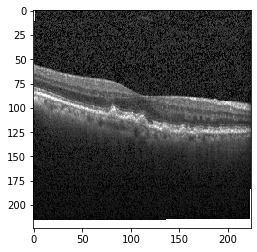
\includegraphics[width=0.2\linewidth]{Assets/prakBMT-DeepLearning-02.png}
    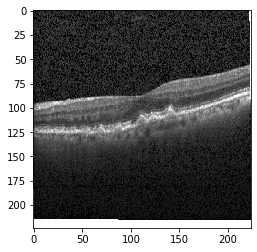
\includegraphics[width=0.2\linewidth]{Assets/prakBMT-DeepLearning-03.png}
    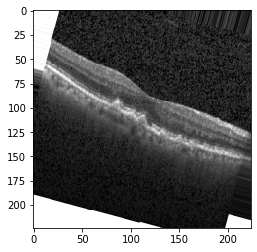
\includegraphics[width=0.2\linewidth]{Assets/prakBMT-DeepLearning-04.png}
\end{center}

\textbf{Antwort:} Spiegelungen und Rotationen können zur Augmentation genutzt werden, da diese keinen Einfluss auf die Diagnose haben. Eine Veränderung der Bilder durch Rauschen oder Helligkeit kann Informationen und Details für das Neuronale Netzwerk unkenntlich machen oder verfälschen.

\subsection{Notebook 3: Grenzen von Deep Learning}
Im Bereich der Medizin spielt Vertrauen in die Technik eine große Rolle. Für das Vertrauen ist es wichtig zu wissen, auf welcher Grundlage die Entscheidungen für eine Klasse getroffen werden. Bisher wurden NN angewendet und sich auf deren Ausgaben verlassen. Die Entscheidungskriterien waren unbekannt. Da NN als ,,Black-Box'' betrachtet werden können, ist dies mit vielen Gefahren verbunden. Diese sollen im Folgenden verdeutlicht werden.

\begin{lstlisting}[language=python]
# Import der benötigten Bibliotheken
exec(open(r"../data/notebook3_code.py").read())
\end{lstlisting}

Es ist ein NN gegeben. Dieses wurde auf einem Datensatz von MRT-Scans trainiert. Diese sehen z.B. wie folgt aus:

\begin{lstlisting}[language=python]
show_mri_example()
\end{lstlisting}
\begin{center}
    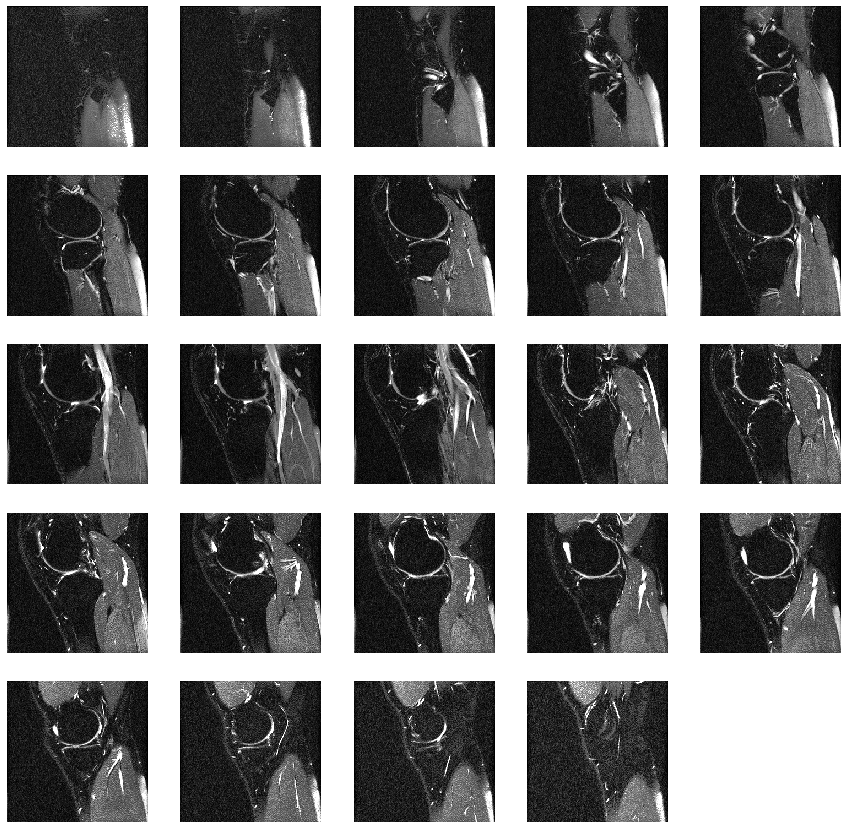
\includegraphics[width=.3\linewidth]{Assets/prakBMT-DeepLearning-05.png}
\end{center}

Je nach Herkunft können die Bilder mit Datumsstempeln oder Wasserzeichen versehen sein. Diese können bei der Anwendung des Netzes später zu Problemen führen.
Die Daten haben die Klassen ,,gesund'' (Klasse 1)  und ,,abnormal'' (Klasse 2). Ein Großteil der als ,,abnormal'' gelabelten Daten stammt von einer (fiktiven) Studie der TU Ilmenau.

Es sind zwei als ,,abnormal'' gelabelte Bilder gegeben.

\begin{lstlisting}[language=python]
# Laden der zwei Bilder
bild1 = []
bild2 = []
path1 = r"../data/mrt_tuil/train/sagittal/0002.npy"
path2 = r"../data/mrt_blank/0008.npy"
#17
a = np.load(path1)
bild1.append(a[int(a.shape[0] / 2)])
b = np.load(path2)
bild2.append(b[int(b.shape[0] / 2)])

bild1 = np.array(bild1, dtype = "float32").reshape(256,256,1)
bild2 = np.array(bild2, dtype = "float32").reshape(256,256,1)

# Speichern der Bilder in einem Array (Praktisch für die Übergabe an keras-Funktionen)
# Array für keras-Funktionen
im_array = np.array([bild1,bild2])
\end{lstlisting}

Die Bilder der als krank diagnostizierten Knie sehen wie folgt aus:
\begin{lstlisting}[language=python]
#Anzeigen der Bilder
plt.figure(1)
plt.title('Bild 1')
plt.axis('off')
plt.imshow(bild1[:,:,0],cmap='jet')
plt.figure(2)
plt.title('Bild 2')
plt.axis('off')
plt.imshow(bild2[:,:,0],cmap='jet')
\end{lstlisting}
\begin{center}
    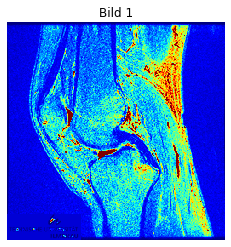
\includegraphics[width=.2\linewidth]{Assets/prakBMT-DeepLearning-06.png}
    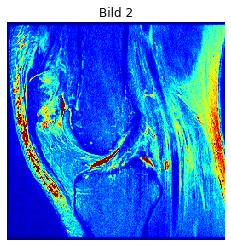
\includegraphics[width=.2\linewidth]{Assets/prakBMT-DeepLearning-07.png}
\end{center}

Nun wird das oben erwähnte NN geladen.

\begin{lstlisting}[language=python]
model= tf.keras.models.load_model(r"../data/mrt.h5")
\end{lstlisting}

Führe nun eine Klassifikation der obigen Bilder durch. Das NN verwendet einen Softmax-Output.

\begin{lstlisting}[language=python]
# TODO: Führen Sie die Klassifikation durch
result = model.predict(im_array)
print("Bild0 = "+str(np.argmax(result[0])))
print("Bild1 = "+str(np.argmax(result[1])))
\end{lstlisting}
Ergebnis:
\begin{lstlisting}[language=python]
    Bild0 = 1
    Bild1 = 0
\end{lstlisting}

Bei diesem Ergebnis ist Skepsis geboten! Interpretiere das Ergebnis.

\textbf{Antwort:} beide Knie sind abnormal. Das NN klassifiziert jedoch eines als Normal. Problematisch wird der unterschiedliche Ausschnitt sein, sowie weniger/mehr rot-gekennzeichnete Zonen.

Im Folgenden soll untersucht werden, worauf das NN seine Entscheidung stützt. Dazu wird der Class Activation Map (CAM)-Algorithmus verwendet. Dieser ordnet einem Bild eine Heatmap zu, welche die Wichtigkeiten der Pixel für die Klassifikationsentscheidung angibt.
Nutze dafür die im Praktikum zur Verfügung gestellte visualize\_class\_activation\_map-Funktion. Diese gibt die zu einem Inputbild gehörende Heatmap der Wichtigkeiten aus.

\begin{lstlisting}[language=python]
# Berechnen der Heatmaps für die zwei Bilder
Map1 = visualize_class_activation_map(model,im_array, img_num=0,klasse=1)
Map2 = visualize_class_activation_map(model,im_array, img_num=1,klasse=0)

# Visualisieren Sie die Heatmaps
plt.figure(1)
plt.title('Bild 1')
plt.axis('off')
plt.imshow(bild1[:,:,0], cmap = "gray")
plt.imshow(Map1, cmap="jet", alpha = 0.4)
plt.figure(2)  
plt.title('Bild 2')
plt.axis('off')
plt.imshow(bild2[:,:,0], cmap = "gray")
plt.imshow(Map2 ,cmap="jet", alpha = 0.4)
\end{lstlisting}
\begin{center}
    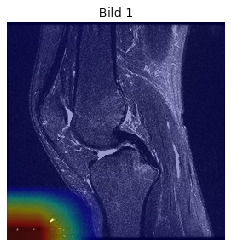
\includegraphics[width=.2\linewidth]{Assets/prakBMT-DeepLearning-08.png}
    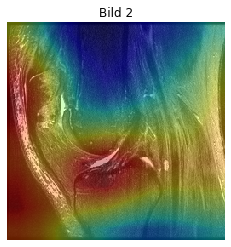
\includegraphics[width=.2\linewidth]{Assets/prakBMT-DeepLearning-09.png}
\end{center}

Was fällt an den beiden Bildern auf? Geben im Protokoll an, auf welches Problem die erste Heatmap hinweist.

\textbf{Antwort:} In Bild 1 ist das Knie nicht betrachtungspunkt des NN. In Bild 2 wird das Knie, besonders der untere Knochen und der vordere Teil, in die Betrachtung mit einbezogen. D.h. bei Bild 1 wird eine völlig falsche Stelle untersucht und für die Diagnose verwendet. Möglicherweise sind Bilddaten falsch interpretiert oder Präperiert worden.

Häufig lassen sich problematische Sachverhalte durch simplere Methoden aufklären.

Die Verwendung einer anderen Colormap kann weitere Informationen ersichtlich machen. Führe den oben verwendeten plt.imshow-Befehl dazu mit anderen Colormaps aus. Können mit einer anderen Colormap das Problem, welches bei diesem NN vorliegt, besser verdeutlicht werden? Erzeuge einen Screenshot für die Colormaps ,,summer'', ,,flag'' und ,,rainbow''.

\begin{lstlisting}[language=python]
# TODO: Untersuchen Sie andere Colormaps
# Führen Sie die Zelle zunächst wie vorgegeben aus und ändern Sie dann die Colormap
plt.figure(1)
plt.title('Bild 1')
plt.axis('off')
plt.imshow(im_array[0,:,:,0],cmap="summer")
plt.figure(2)
plt.title('Bild 2')
plt.axis('off')
plt.imshow(im_array[1,:,:,0],cmap="summer")
\end{lstlisting}
\begin{center}
    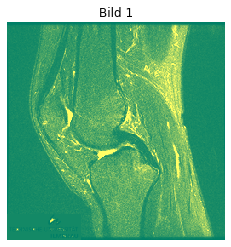
\includegraphics[width=.2\linewidth]{Assets/prakBMT-DeepLearning-10.png}
    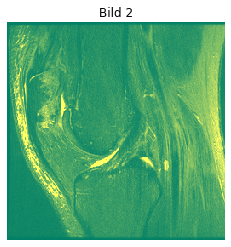
\includegraphics[width=.2\linewidth]{Assets/prakBMT-DeepLearning-11.png}
\end{center}

\begin{lstlisting}[language=python]
plt.figure(1)
plt.title('Bild 1')
plt.axis('off')
plt.imshow(im_array[0,:,:,0],cmap="flag")
plt.figure(2)
plt.title('Bild 2')
plt.axis('off')
plt.imshow(im_array[1,:,:,0],cmap="flag")
\end{lstlisting}
\begin{center}
    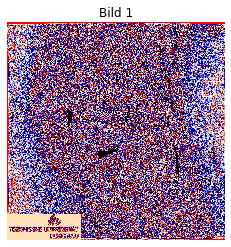
\includegraphics[width=.2\linewidth]{Assets/prakBMT-DeepLearning-12.png}
    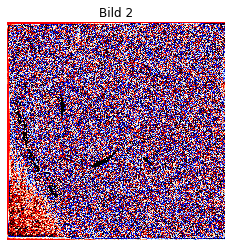
\includegraphics[width=.2\linewidth]{Assets/prakBMT-DeepLearning-13.png}
\end{center}

\begin{lstlisting}[language=python]
plt.figure(1)
plt.title('Bild 1')
plt.axis('off')
plt.imshow(im_array[0,:,:,0],cmap="rainbow")
plt.figure(2)
plt.title('Bild 2')
plt.axis('off')
plt.imshow(im_array[1,:,:,0],cmap="rainbow")
\end{lstlisting}
\begin{center}
    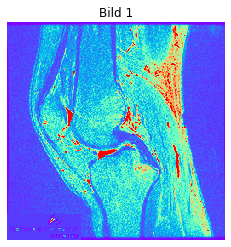
\includegraphics[width=.2\linewidth]{Assets/prakBMT-DeepLearning-14.png}
    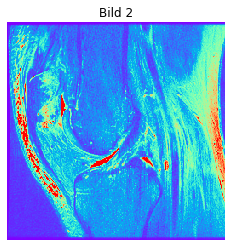
\includegraphics[width=.2\linewidth]{Assets/prakBMT-DeepLearning-15.png}
\end{center}

Lösung: Die TU Ilmenau hat die Daten mit einem Schriftzug unten links versehen. Das Netz hat gelernt, im Falle kranker Knie auf diese zu achten.

\end{document}

